\begin{exo}{}
	On considère le tableau de variations d'une fonction $f$ :

	\begin{center}
		\begin{tikzpicture}
			\tikzset{arrow style/.style={->, >=Triangle, thick}}
			\tkzTabInit[lgt=1,espcl=1.5]{$x$ / 0.7 , $f$ / 1.3}{$-\infty$, $-2$, $1$, $5$}
			\tkzTabVar{-/ , +/ $5$ , -/ $3$ , +/ $4$}
		\end{tikzpicture}
	\end{center}

	\begin{enumerate}
		\item Préciser l'ensemble de définition $\mathcal{D}$ de $f$.
		\item En utilisant les termes « croissante » et « décroissante », décrire les variations de $f$.
		\item Peut-on affirmer que :
		      \begin{enumerate}
			      \item $5$ est le maximum de $f$ sur $\mathcal{D}$ ?
			      \item $3$ est le minimum de $f$ sur $\mathcal{D}$ ?
		      \end{enumerate}
		\item Comparer, en justifiant, les nombres suivants :
		      \begin{enumerate}
			      \item $f(-10)$ et $f(-5)$
			      \item $f(0)$ et $f(1)$
			      \item $f(2)$ et $f(3)$
		      \end{enumerate}
		\item Est-il possible de comparer $f(-4)$ et $f(0)$ ? Justifier.
		\item Quelles sont toutes les images que l'on peut comparer à $f(1)$ ?
		\item Dans un repère orthonormé, tracer une possible courbe représentative de $f$.
	\end{enumerate}
\end{exo}
